\section{Give a definition of refactoring in your own words and illustrate it with a concrete example of a
refactoring.}

A refacotring is a software transformation that
\begin{itemize}
\item preserves the external behavior of the software
\item improves the internal structure of the software
\end{itemize}

In other words, refactoring is a disciplined way to clean up code that minimises the chances of introducing bugs. It has also the purpose to make the software easier to understand \textbf{and} modify.
\\For example, the following code: \\
 \begin{lstlisting}[caption=before refactoring]
class AwesomeAddon {

    private Settings [] settings;

    public AwesomeAddon (Settings settings ) {
        this.settings = settings;
    }
    protected function set_settings(Settings settings ) {
        if ( notAnArray( this.settings ) ) {
            throw new Exception( 'Invalid settings' );
        }
        this.settings = settings;
    }
    protected function do_something_awesome() {
        //...
    }
}


class EvenMoreAwesomeAddon {

    private Settings [] settings;

    public EvenMoreAwesomeAddon (Settings settings ) {
        this.settings = settings;
    }
    protected function set_settings(Settings settings ) {
        if ( notAnArray( this.settings ) ) {
            throw new Exception( 'Invalid settings' );
        }
        this.settings = settings;
    }
    protected function do_something_even_more_awesome() {
        //...
    }
}
\end{lstlisting}
Becomes : \\
\begin{lstlisting}[caption=after refactoring]
abstract class Addon {
    protected Settings [] settings;
    protected function set_settings( Settings settings ) {
        if ( notAnArray( settings ) ) {
            throw new Exception( 'Invalid settings' );
        }
        this.settings = set_settings(settings);
    }
}

class AwesomeAddon extends Addon {

    public AwesomeAddon(Settings settings ) {
        this.settings = set_settings(settings);
    }
    protected function do_something_awesome() {
        //...
    }
}

class EvenMoreAwesomeAddon extends Addon {

    public EvenMoreAwesomeAddon( $settings ) {
        this.settings = set_settings(settings);
    }
    protected function do_something_even_more_awesome() {
        //...
    }
}
\end{lstlisting}
\section{Explain why it is important to refactor.}
it is important to refactor in order to:

\begin{itemize}
\item improve the software's design
\item counter code decay (software aging). It helps code to remain in shape.
\item increase the software's comprehensibility
\item find bugs and write more robust code
\item increase productivity (on long term basis only).
\item To reduce costs of software maintenance
\item reduce testing
\item facilitate future customisations
\item To turn an Object Oriented application into a framework
\item introduce design patterns in a behaviourally preserving way
\end{itemize}

\section{Explain when refactoring should (or should not) be performed.}

\subsection{When should we refactor?}

\begin{itemize}
\item Whenever we see the need for it
\begin{itemize}
\item Do it all the time in little bursts
\item Not on a pre-set periodical basis
\end{itemize}
\item Apply the rule of three
\begin{itemize}
\item Implement from scratch
\item implement something similar by code duplication
\item do not implement similar things again, but refactor
\end{itemize}
\item Refactor when adding new features or functions (Especially if  feature is difficult to integrate with the existing 
code )
\item Refactor during bug fixing 
\begin{itemize}
\item If  a bug is very hard to trace, refactor first to make the code more understandable, so that you can understand better 
where the bug is located
\end{itemize}
\item Refactor during code reviews
\item bonus :\\
\begin{itemize}
\item Refactoring also fits naturally in the agile methodsphilosophy 
\item Refactoring is needed to address the principle "Maintain 
simplicity". Wherever possible, actively work to eliminate complexity from the system by refactoring the code
\end{itemize}
\end{itemize}

\subsection{When shouldn't we refactor?}
\begin{itemize}
\item When the existing code is such a mess that although you could refactor it, it would be easier to rewrite everything from scratch instead. 
\item When you are too close to a deadline because the productivity gain would appear after the deadline and thus be too late. 
\end{itemize}
However,you should never put off refactoring (if not too close frome deadline) because you don’t have the time. Not having enough time usually is a sign that refactoring is needed.
\section{Like refactoring, performance optimisation does not usually change the behaviour of the code
(other than its speed); it only alters the internal structure. So how does it differ from refactoring
then?}

Refactoring typically changes no functionality, it simply changes the code's form to make the code more understandable and maintainable, e.g. by hiding parts of it behind interfaces in order to make it exchangable.
\\
Optimization typically changes the performance of a functionality, e.g. making execution faster or memory footprint smaller.\\
Refactoring is not performance optimization. However, a peculiar indirect side effect of refactoring is probably more efficient resource usage.

\section{Explain and illustrate the Extract Method refactoring.}
 The Extract method is used when you have a fragment of code that can be grouped together, turn it into a method with a name that explains the purpose of the method. This method helps to improve clarity and remove redundancy .
 \\
 We can illustrate this method as follows :\\
 \begin{lstlisting}[caption=Without extract method]
public void accept(Packet p) { 
	if ((p.getAddressee() == this) && (this.isASCII(p.getContents()))) //Fragment to extract
		this.print(p); 
	else  
		super.accept(p); 
}
\end{lstlisting}

\begin{lstlisting}[caption=With extract method]
public void accept(Packet p) {
	if this.isDestFor(p)
    	this.print(p); 
	else
    	super.accept(p); 
}

public boolean isDestFor(Packet p) {
	//Fragment extracted 
	return ((p.getAddressee() == this) && (this.isASCII(p.getContents())));
}
\end{lstlisting}

\section{Same question as previous one but for one of the following refactorings:
Move Method, Extract Class, Replace Type Code with Subclass,
Replace Subclass with Fields, Pull Up Method, Introduce Parameter Object}
\subsection{Move Method(resp. field)}
The move method refactoring is used When a method (resp. field) is used by or uses more features of another class than its own, create a similar method (resp. field) in the other class; remove or delegate original method (resp. field) and redirect all references to it. This refactor method is the essence of refactoring.\\
\textbf{Example}:

\begin{figure}[!ht]
\centering
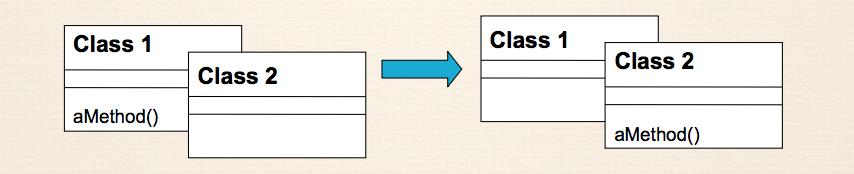
\includegraphics[scale=0.8]{movemethod.png}
\caption{Move Method example}
\end{figure}
\FloatBarrier{}

\subsection{Extract Class}
The extract class refactoring method is used when you have a class doing work that should be done by two,create a new class and move the relevant fields and methods to the new class. The idea is to avoid too large classes that are hard to understand.\\
\textbf{Example}:

\begin{figure}[!ht]
\centering
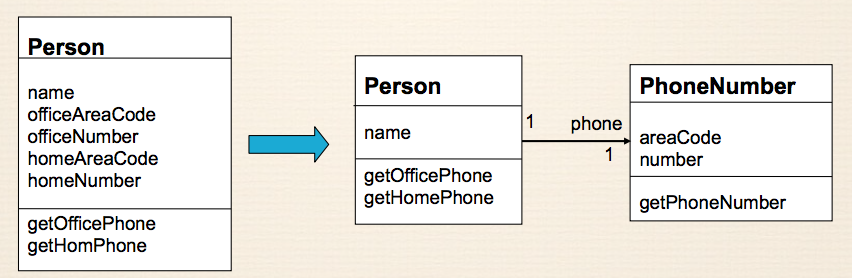
\includegraphics[scale=0.8]{extractclass.png}
\caption{Extract class example}
\end{figure}
\FloatBarrier{}

\subsection{Replace Type Code with subclass}
This replacement is used when there are immutable type code that affect the behaviour of a class. Instead of having lots of immutable variables to represent the type of the object, create subclasses that represents the different object.\\
\textbf{Example}:

\begin{figure}[!ht]
\centering
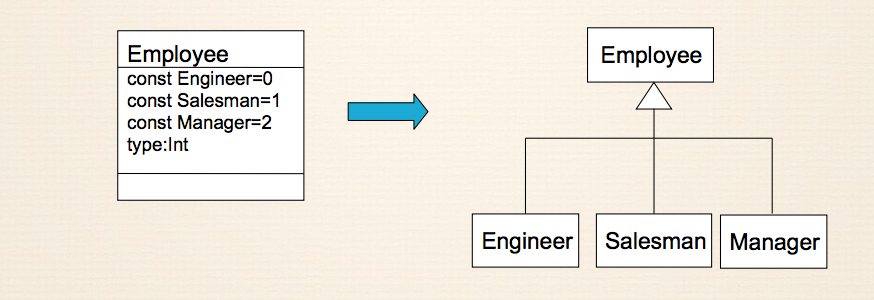
\includegraphics[scale=0.8]{replacetype.png}
\caption{Replace Type Code with subclass example}
\end{figure}
\FloatBarrier{}


\subsection{Replace subclass with Fields}
This method is the opposite of the Replace Type Code with subclasses. Subclasses vary only in methods that return constant data. We just need to change methods to superclass fields and eliminate subclasses.\\
\textbf{Example}:

\begin{figure}[!ht]
\centering
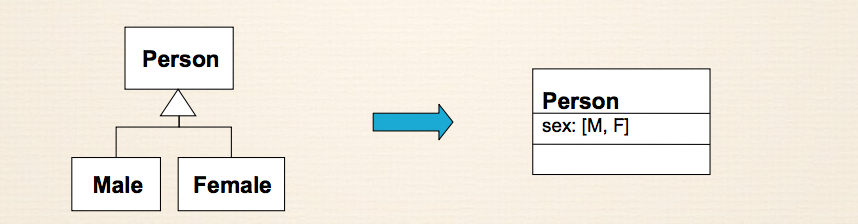
\includegraphics[scale=0.8]{replacefields.png}
\caption{Replace subclass with fields example}
\end{figure}
\FloatBarrier{}

\subsection{Pull up Method}
There are two variants of this method. The first one (simple one) consist of looking for methods with same name in subclasses that do not appear in superclass.\\
The other one (more complex) focus more on the behaviour of the method.\\
If the method that is being pulled up already exists in the superclass as an abstract method, make it
concrete with the common behaviour.
\\
\textbf{Example}:

\begin{figure}[!ht]
\centering
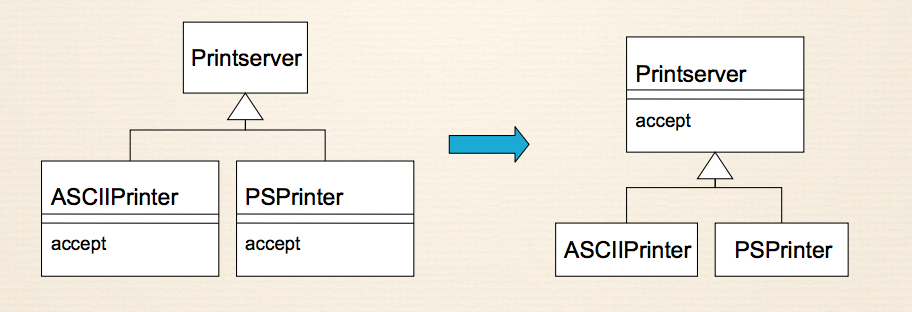
\includegraphics[scale=0.8]{pullup.png}
\caption{Pull-up Method example}
\end{figure}
\FloatBarrier{}

\subsection{Introduce Parameter Object}
The purpose here is quite simple : group parameters that belong together in a separate object.
\\
\textbf{Example}:

\begin{figure}[!ht]
\centering
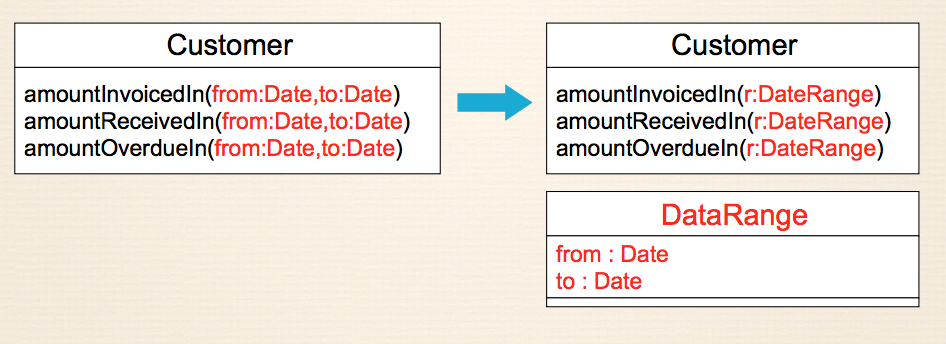
\includegraphics[scale=0.8]{parameterobject.png}
\caption{Introduce Parameter Object example}
\end{figure}
\FloatBarrier{}


\section{Give a concrete example of how a refactoring could accidentally reduce quality.}

When we don't know what we are doing and when refactoring is not applied correctly, it can decrease the quality of the code. For exemple, going too deep in the abstraction.\\
Refactoring should remove bad smells and not add new ones.

\textbf{Example}: Too abstract class

\begin{figure}[!ht]
\centering
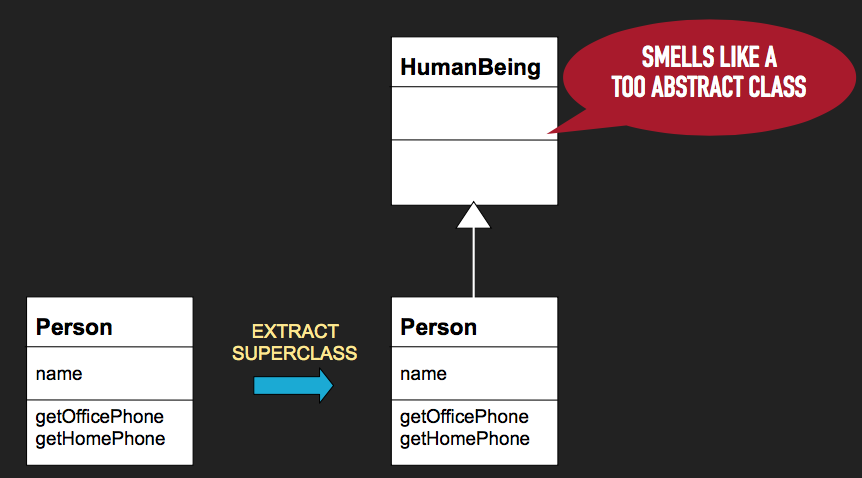
\includegraphics[scale=0.8]{tooabstract.png}
\caption{Too abstract class example}
\end{figure}
\FloatBarrier{}

\section{Give an example of how to independently applied refactorings could accidentally introduce a
subtle merge conflict.}

\begin{figure}[!ht]
\centering
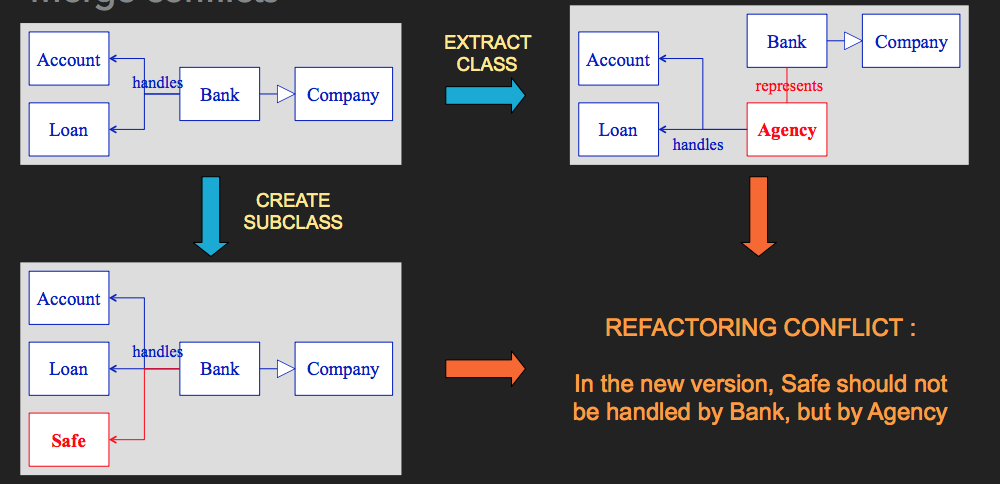
\includegraphics[scale=0.8]{merge_conflict.png}
\caption{Merge conflict example}
\end{figure}
\FloatBarrier{}
